%% Hello emacs, this is -*- latex -*-
\typeout{ ====================================================================}
\typeout{ This is file trigger.tex, created at 28-Feb-2004 }
\typeout{ Maintained by Andre dos Anjos <Andre.dos.Anjos@cern.ch> }
\typeout{ ====================================================================}

\chapter{O Sistema de filtragem e aquisição de dados do ATLAS}
\label{chap:trigger}

O \idx{sistema de filtragem} do experimento ATLAS tem o encargo de separar
\eng{online} a Física considerada como ordinária segundo o experimento, dos
raros eventos de interesse. A taxa de eventos produzida pelo LHC será de 40
milhões por segundo, ou 40 MHz, em bateladas que durarão cerca de 10 horas
(este período é comumente referido como \eng{run}). Cada evento poderá
produzir uma colisão favorável à Física de interesse, embora a grande maioria,
mais de 99,9999\%, represente canais físicos já bastante estudados em
experimentos anteriores, ainda que a luminosidade do sistema seja tão
elevada. Ademais, cada evento detetado pelo ATLAS produzirá cerca de 1,5
Megabyte em dados, o que torna o problema da filtragem bastante difícil, já
que o fluxo de dados que deve ser analisado por base de tempo está acima da
capacidade de qualquer tecnologia de transporte de dados atual.

Para o experimento ATLAS, o sistema de filtragem será construído em 3 níveis
seqüenciais (veja a Figura~\ref{fig:trigger-sketch}). Cada nível que se sucede
refina a decisão do nível anterior através da aquisição de mais dados do
detetor. O Primeiro Nível de filtragem (do inglês \eng{First-Level Trigger},
\gls{glos:lvl1}), deverá reduzir a taxa de eventos do LHC para cerca de 100
kHz apenas, através de técnicas simples de filtragem codificadas em
\eng{hardware} dedicado. O Segundo Nível de Filtragem (do inglês
\eng{Second Level Trigger}, \gls{glos:lvl2}), reduzirá a taxa de saída do LVL1 para
aproximadamente 1 kHz utilizando aplicações codificadas em
\eng{software} para computadores do tipo PC, tão comuns quanto os disponíveis
para aplicações domésticas. O Filtro de Eventos (do inglês \eng{Event Filter},
\gls{glos:ef}), estará baseado na mesma tecnologia escolhida para o LVL2,
reduzindo a taxa de entrada de eventos para aproximadamente 100 Hz, através de
algoritmos de filtragem mais eficientes, porém mais lentos. Os eventos
ultimamente selecionados pelo EF são armazenados em mídia permanente, para
posterior análise \eng{offline}. 

\begin{figure}
\begin{center}
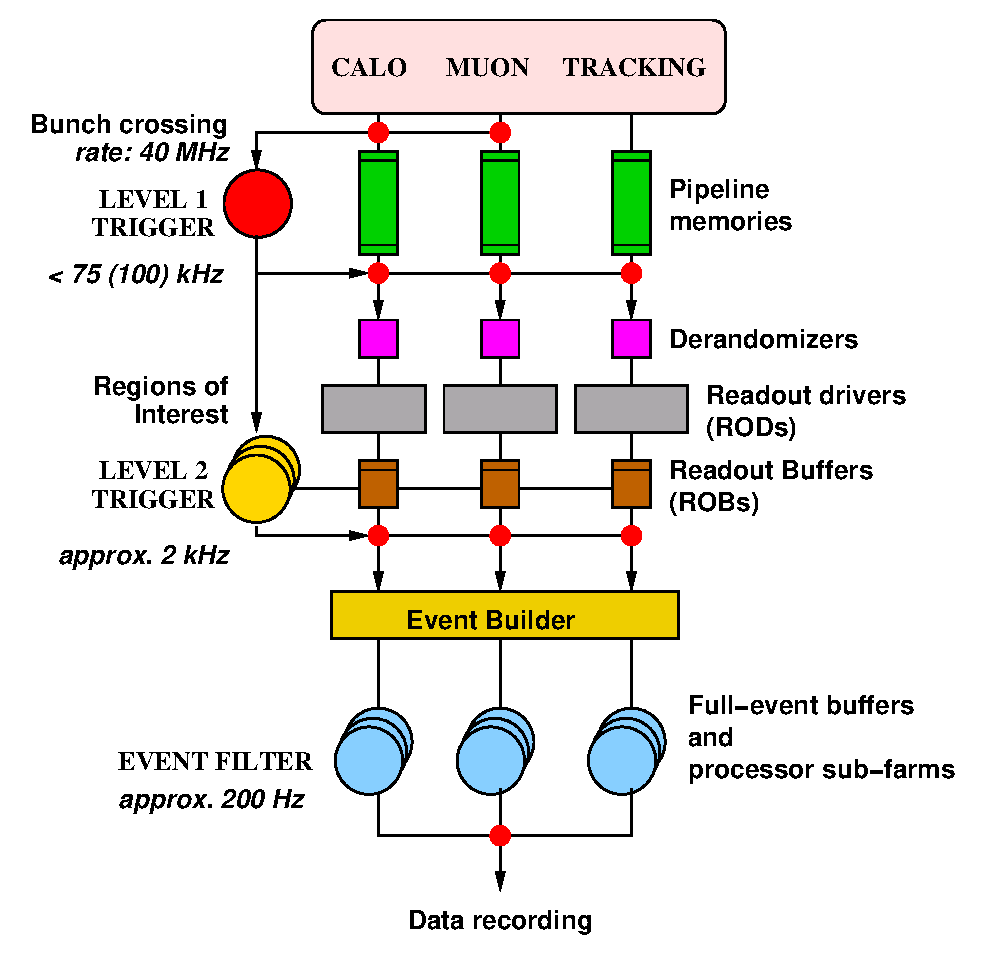
\includegraphics[angle=-90,scale=0.8]{trigger-sketch}
\end{center}
\caption[Visão funcional simplificada do sistema de filtragem do experimento
ATLAS.]{Visão funcional simplificada do sistema de filtragem do experimento
ATLAS. Extraído de \cite{hlt-tdr}.}
\label{fig:trigger-sketch}
\end{figure}

\section{O primeiro nível de filtragem}
\label{sec:lvl1}

O LVL1 realiza uma seleção inicial de candidatos à Física de interesse baseada
em informações com segmentação reduzida, fornecidas por um subconjunto dos
detetores do ATLAS, os calorímetros e os detetores de múons
\cite{l1-tdr}. Múons com altos valores de \idx{momento transverso} ($p_T$) são
identificados a partir das câmaras de trigger conectadas ao Espectrômetro de
Múons (veja a Seção~\ref{sec:atlas-muon}) na região do barril e da tampa. As
seleções baseadas em calorimetria utilizam uma segmentação reduzida das seções
e.m. e hadrônica no barril e na tampa. Os objetos procurados usando-se
calorímetros no LVL1 são elétrons com altos valores de $p_T$ e fótons, jatos,
taus decaindo em cascatas hadrônicas, grandes quantidades de energia faltante
ou energia transversa total. No caso da seleção de elétrons e fótons ou
hádrons e taus, isolamento em energia\footnote{Isolamento em energia significa
a ausência de outros picos energéticos adjacentes ao pico energético sendo
analisado.} pode ser requisitado.

Para gerar os sinais de filtragem necessários ao LVL1, o sistema de leitura de
dados dos calorímetros é equipado com somadores rápidos \cite{seixas:adder,
lar-tdr} que aglomeram o sinal de 2 ou mais células destes detetores para
gerar macro-células de filtragem denominadas \idx{torres de filtragem} (do
inglês \idxeng{Trigger Towers}, \gls{glos:tt}). O sistema de múons também possui
circuitos equivalentes que determinam a ocorrência de traços com altos valores
de momento transverso ($p_T$) naquele subdetetor.

Os eventos selecionados pelo LVL1 são lidos a partir da eletrônica específica
de cada detetor por meio de \eng{drivers} denominados \eng{ReadOut Drivers}
(\gls{glos:rod}'s). Cerca de 1.600 ROD's serão necessários para ler todos os
dados do detetor, ou seja, aproximadamente $10^7$ canais independentes. Vários
canais de leitura são multiplexados em cada ROD. Bancos de memória primários,
chamados de \eng{derandomizers}, garantem um fluxo contínuo dos dados aos
ROD's, apesar da irregularidade da aceitação de eventos proporcionada pelo
LVL1.

Os dados completos de eventos selecionados são guardados momentaneamente em
bancos de memória denominados \eng{ReadOut Buffers} (\gls{glos:rob}'s) até que
o evento seja rejeitado pelo LVL2 ou, no caso de ser aceito por este nível,
até que os dados sejam transferidos para o terceiro nível de filtragem (EF). O
processo de mover os dados dos ROB's para o EF é chamado de \idx{construção do
evento} (do inglês, \idxeng{Event Building}, \gls{glos:eb}). Porém, até a fase de
construção do evento, os dados estarão segmentados em ROB's. Após esta etapa,
o evento completo estará guardado em um único banco de memória e acessível a
um processador do EF. 

\paragraph{Regiões de Interesse} Além do disparo dado pelo LVL1 à eletrônica de
leitura, este nível de filtragem deve enviar ao LVL2 um mapa dos objetos de
interesse encontrados no detetor durante a avaliação do evento. Este mapa
indica, na precisão do LVL1, as \idx{regiões de interesse} no detetor (do inglês
\eng{Region of Interest}, \gls{glos:roi}) que contribuíram para a seleção, os tipos
de objetos encontrados e o valor mínimo (\eng{threshold}) de $p_T$ que
satisfazem. Informações de RoI's secundárias (que não contribuíram para a
decisão do LVL1, mas que excitaram notavelmente o detetor) também podem ser
transmitidas ao LVL2, provendo maior flexibilidade de decisão a este nível.

Na Figura~\ref{fig:l1-context}, é possível observar um diagrama do tipo
``caixa-preta'', indicando os sinais de entrada e saída do LVL1. A este
sistema são injetados os sinais provenientes da eletrônica de leitura e dos
sistemas de filtragem diretamente acoplados aos detetores e do LHC
(\eng{clock} de 40 MHz). Deste sistema serão colhidos sinais que serão, por
sua vez, encaminhados para o LVL2, para a eletrônica de aquisição e para o
sistema de monitoração central.

\begin{figure}
\begin{center}
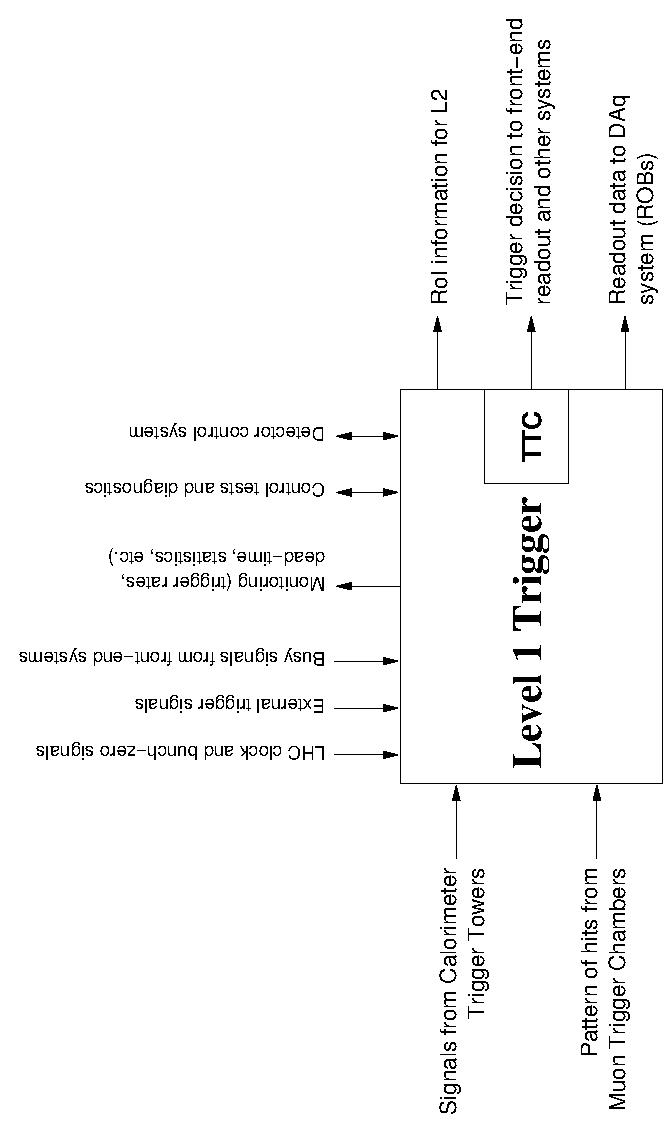
\includegraphics[scale=0.75,angle=-90]{l1-blackbox}
\end{center}
\caption[Diagrama simplificado dos sinais de entrada e saída do
LVL1.]{Diagrama simplificado dos sinais de entrada e saída do
LVL1. Extraído de \cite{hlt-tdr}.}
\label{fig:l1-context}
\end{figure}

Na Figura~\ref{fig:l1-functional} observa-se um diagrama funcional
simplificado do LVL1. Nesta figura é possível identificar processadores
específicos para os sinais provenientes dos detetores. Um \idx{processador
central de filtragem} (marcado na figura como \eng{Central Trigger Processor})
é responsável pela decisão final e pela emissão do sinal para o LVL2 e para o
sistema de distribuição de tempo, disparo e controle (indicado como
\eng{Timing, Trigger and Control distribution}, ou \gls{glos:ttc}), que gera,
finalmente, o sinal para a leitura dos dados do detetor. Dentre os componentes
do TTC está o \idx{Construtor de RoI's} (do inglês \idxeng{RoI Builder}, RoIB)
que monta o mapa de RoI's destacadas pelo LVL1 e comunica, através de uma
conexão serial rápida tipo S-Link, estes dados ao LVL2.

\begin{figure}
\begin{center}
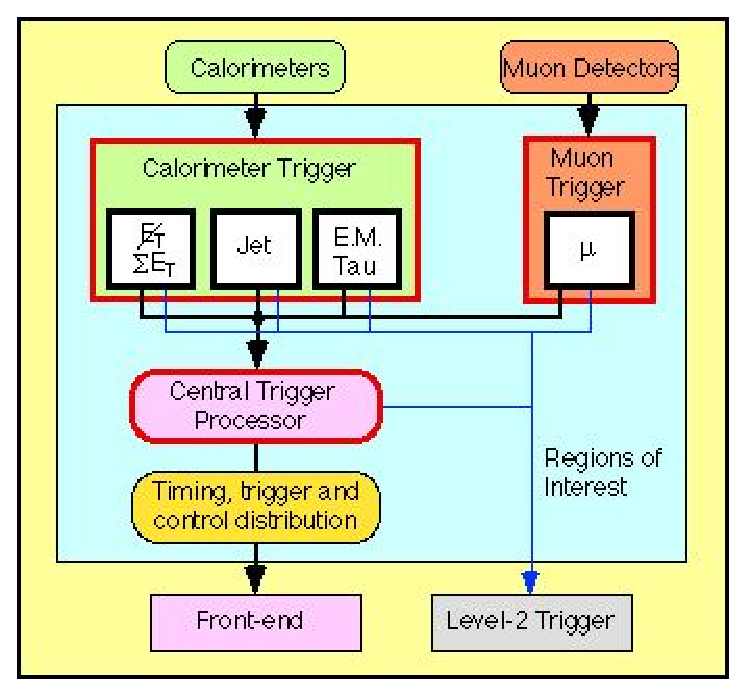
\includegraphics[scale=0.8]{l1-functional}
\end{center}
\caption[Diagrama em blocos indicando as principais funções do LVL1.]{Diagrama
em blocos indicando as principais funções do LVL1. Extraído de \cite{hlt-tdr}.}
\label{fig:l1-functional}
\end{figure}

\section{Os altos níveis de filtragem, aquisição de dados e controle}
\label{sec:hlt-daq}

%% Observação: falta referência para S-Links

O \idx{sistema de aquisição de dados} do ATLAS (do inglês \idxeng{Data
Acquisition System}, \gls{glos:daq}) é composto por processadores que estão
encarregados da transmissão e manipulação dos dados produzidos pelo detetor
\cite{hlt-tdr}. O DAQ trabalha em cooperação com os diversos níveis de
filtragem e controle do experimento, de forma a garantir a correção dos dados
transmitidos e a minimização do tempo morto despendido no tráfego de
informação pelo sistema. A cadeia de operação do DAQ é iniciada por um disparo
do LVL1 para a leitura de dados executada nos ROD's. Cada ROD é ligado,
através de uma conexão S-Link\footnote{Conexão serial ponto-a-ponto com taxa
máxima de transferência de 160 megabits por segundo.}, a somente um ROB. Cada
ROB pode receber dados de um ou no máximo 3 ROD's, dependendo da configuração
final do experimento.

Cabe aos \idx{Altos Níveis de Filtragem} (do inglês \idxeng{High-Level
Triggers}, \gls{glos:hlt}), analisando de forma ótima os dados presentes nos
ROB's, decidir, disparando mais uma vez o DAQ, sobre o futuro de cada evento
aceito pelo LVL1. O conjunto HLT-DAQ-Controle deverá funcionar harmoniosamente
sobre uma mesma base computacional, utilizando ainda o mesmo conjunto de
ferramentas para a codificação, análise e depuração de eventuais problemas que
possam ocorrer. Por esta razão, esta união de produtos de \eng{hardware} e
\eng{software} é considerada um macro-sistema do experimento. Este sistema
pode ser subdividido em 4 partes:

\begin{itemize}
\item \textbf{\idx{Sistema de controle do detetor} ou \eng{Detector Control
System}, \gls{glos:dcs}}: responsável pela operação coerente e segura (no que tange
a radiação, controle de altas tensões, etc.) do detetor ATLAS e pelo
interfaceamento com sistemas externos e serviços incluindo o acelerador
LHC. Uma vez que este tópico não está diretamente envolvido neste trabalho,
será abordado somente em caráter introdutório;

\item \textbf{\eng{Online}}: é responsável por todos os aspectos de
operação e controle durante a aquisição de dados do experimento e durante
operações (\eng{runs}) de teste e calibração;

\item \textbf{\idx{Fluxo de dados} ou \eng{Dataflow}}: este sistema é
responsável por receber os dados do detetor, servir um subconjunto destes
dados ao HLT e transportar os dados de eventos selecionados em última
instância para armazenagem em mídia permanente;

\item \textbf{\idx{Altos Níves de Filtragem} ou \idx{HLT}}: são responsáveis pela
seleção de eventos após o LVL1, envolvendo a redução da taxa de eventos e a
classificação de todos os eventos aceitos.

\end{itemize}

\subsection{O sistema de controle do detetor}
\label{sec:dcs}

O DCS supervisiona todos os componentes de \eng{hardware} do arranjo
experimental, incluindo todos os sistemas de deteção do ATLAS. O DCS também se
comunica com sistemas externos, como a infraestrutura de serviços do CERN e,
mais notavelmente, com o acelerador LHC.

Aspectos de segurança são tratados pelo DCS somente no nível de menor
severidade. Este sistema cuida principalmente de questões ligadas ao
seqüenciamento de operações ou à requisição onde prevaleçam condições
específicas, antes de permitir que outros procedimentos sejam
executados. Ferramentas para a construção de interdependências, tanto em
\eng{hardware} quanto em \eng{software}, são providas pelo DCS. Monitoração e
prevenção de situações que poderiam causar danos maiores ao detetor e à vida
das pessoas são de responsabilidade de sistemas dedicados - o \idx{Sistema de
Segurança do Detetor} (do inglês \eng{Detetor Safety System}, \gls{glos:dss}) e
do sistema de segurança e alarme do CERN respectivamente. O DCS interage com
ambos os sistemas.

Todas as ações iniciadas pelo operador e todos os erros, avisos e alarmes que
impliquem em falha de \eng{hardware} do detetor são gerenciadas pelo DCS. Este
sistema provê informação \eng{online} da situação presente, com a
granularidade necessária para uma operação centralizada do sistema. A
interação dos \eng{experts} em detetores com suas máquinas também é feita
através do DCS, que continuamente monitora todos os parâmetros operacionais,
guiando o operador e sinalizando qualquer comportamento anormal do
maquinário. O DCS também será capaz de acionar procedimentos automáticos para
trazer o sistema de deteção para um estado seguro, se necessário for.

No que tange à operação do experimento, a interação com o sistema de aquisição
de dados é de grande importância. A boa qualidade da Física gravada em mídia
permanente depende de uma sincronização absoluta entre o DAQ e o DCS; ambos os
sistemas são complementares. O DAQ lida com eventos caracterizados por números
e o DCS guarda o estado operacional do detetor enquanto os dados estão sendo
adquiridos, correlacionando os números dos eventos com a qualidade da
aquisição, que, finalmente, é avaliada \eng{offline}.

Algumas partes do detetor operarão continuamente, pois qualquer interrupção
pode ser custosa em tempo, fundos ou desempenho do sistema global. Portanto, a
supervisão do sistema de deteção é necessária constantemente. Por outro lado,
o DAQ é somente necessário durante a aquisição de dados ou durante \eng{runs}
de monitoração, calibração ou teste. Assim sendo, o DCS precisa ter completa
independência funcional, ainda que, ao mesmo tempo, este quesito não deva,
imperativamente, acarretar em limites operacionais com o DAQ.

\subsection{O sistema \textit{online}}
\label{sec:online}

O sistema \idxeng{online} engloba o conjunto de aplicações para configurar,
controlar e monitorar o sistema de filtragem e aquisição de dados do ATLAS (do
inglês \eng{Trigger and Data Acquisition}, \gls{glos:tdaq}), excluindo o
gerenciamento, processamento e transporte de dados físicos. É um conjunto
personalizável de ferramentas que provê a ``cola'' que une entradas e saídas
dos outros sistemas. O sistema \eng{online} não contém elementos que sejam
específicos aos detetores, pois é também utilizado por todos os sistemas de
instrumentação da aquisição de dados de forma transparente. Ele coopera com
outros sub-sistemas e interfaces para a leitura do detetor, DCS, LVL1,
\eng{Dataflow}, HLT, \eng{Offline} e o interfaceamento com operadores dos
\eng{runs}.

Um dos papéis importantes do sistema \eng{online} é prover serviços para guiar
o TDAQ na sua inicialização e finalização, de forma que os aplicativos sejam
executados de maneira ordenada. Este sistema é responsável pela sincronização
dos estados de um \eng{run} para todo o sistema de filtragem, aquisição e
supervisão. Os procedimentos de ligamento e desligamento são projetados para
se alcançar o menor tempo possível, reduzindo tempos-mortos, pois isto afeta
diretamente a quantidade de dados que podem ser adquiridos em um período de
funcionamento do LHC. Ferramentas de verificação e diagnóstico ajudam a
detetar problemas de maneira precoce e eficiente. Bancos de dados com a
configuração do sistema são fornecidos contendo um grande número de parâmetros
que descrevem a topologia do sistema, os componentes de
\eng{hardware} e \eng{software}, assim como os modos e ordem de
execução. Durante a aquisição, componentes especializados capturam e servem
dados relacionados à monitoração dos diversos processos do experimento, tais
como histogramas e parâmetros de rejeição, assim como mensagens de erro e
diagnóstico enviadas pelas diversas aplicações. Interfaces (gráficas) aos
operadores permitem configurar e controlar diversas funcionalidades do
experimento. Estas interfaces fornecem visões simplificadas de vários
sub-sistemas durante um \eng{run}.

\subsubsection{Arquitetura do sistema \eng{online}}
\label{sec:online-arch}
\index{online}

O projeto do sistema \eng{online} é baseado numa arquitetura de componentes,
que respeitam o modelo cliente-servidor. Os componentes podem ser divididos em 3
grupos, que incluem um conjunto de pacotes cada um. Cada um dos pacotes está
associado a um grupo de funções para este sistema, e provê um conjunto definido
de serviços. Os serviços possuem interfaces bem definidas e são desacoplados
entre si.

\paragraph{Controle:} contém pacotes para o controle do sistema de
aquisição, filtragem e deteção. Os pacotes de controle existem para propiciar
ao TDAQ capacidades de inicialização e finalização, distribuição de comandos,
sincronização, manuseio de erros e verificação do sistema.

O sistema de controle de dispositivos e aplicações do sistema \eng{online} é
baseado em uma \idx{máquina de estados finitos} global mostrada na
figura~\ref{fig:online-fsm}. Todos os dispositivos do sistema devem
obedecê-la, enviando avisos e erros caso falhem em cumprir as ordens do
operador.

\begin{figure}
\begin{center}
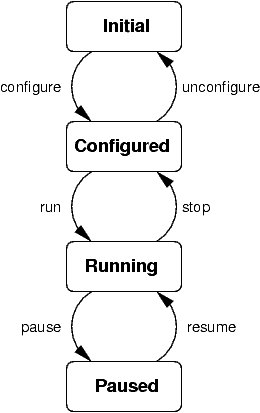
\includegraphics[scale=0.7]{online-fsm}
\end{center}
\caption{A máquina de estados finitos utilizada por todos os componentes do
TDAQ e detetores do ATLAS.}
\label{fig:online-fsm}
\end{figure}

Este pacote também provê uma interface gráfica, escrita em Java, para o
acionamento e verificação de todas as partes do sistema de filtragem e
aquisição de dados, indicando prontamente problemas, ou encaminhando avisos ao
operador do \eng{run}.

%Na Figura~\ref{fig:playdaq} é possível ver algumas
%imagens desta interface. A imagem na parte superior mostra a janela de
%controle central. Outras abas existem e podem ser utilizadas para acessar
%outras informações, como o estado do equipamento ou a taxa de operação de cada
%processador do sistema.

%\begin{figure}
%\begin{center}
%
\includegraphics[scale=1]{missing}
%\end{center}
%\caption{Algumas janelas da interface ao usuário do Sistema \eng{online}.}
%\label{fig:playdaq}
%\end{figure}

\paragraph{Bancos de dados:} contêm pacotes para a \idx{configuração} do TDAQ e
detetores. Os pacotes de configuração existem para propiciar parâmetros de
configuração do sistema, sua descrição e acesso e registro operacional de
informações durante a aquisição de dados. Há também componentes que provêem
acesso de leitura e escrita a bancos de dados que descrevem as condições do
feixe provido pelo LHC e do detetor.

Como no caso do pacote de controle, existem ferramentas para a manipulação e
verificação dos bancos de dados produzidos pelo usuário, que podem facilmente
chegar a dezenas de megabytes em sua versão final, uma vez que englobará a
configuração de milhares de componentes. Atualmente, somente uma das
interfaces de operação a banco de dados está disponível e é baseada na
utilização de arquivos locais, uma vez que o código para o acesso remoto de
bancos de dados não está implementado ainda.

\paragraph{Compartilhamento de informação:} contém pacotes para o
compartilhamento de informação no TDAQ. Os componentes destes pacotes podem
anunciar erros, publicar estados, estatística e histogramas construídos pelos
sub-sistemas do TDAQ e pelos detetores. Há um conjunto de interfaces gráficas
para a monitoração do Sistema de Filtragem do ATLAS, que podem ser acessadas
através da linha de comando em ambientes apropriadamente configurados.

%A Figura~\ref{fig:daqmonitor} exibe uma das possibilidades de
%monitoração. Nesta janela estamos observando algumas aplicações sendo
%processadas em diferentes nós de um sistema de teste.

%\begin{figure}
%\begin{center}
%
\includegraphics[scale=1]{missing}
%\end{center}
%\caption{Uma das interfaces gráficas do sistema de monitoração do DAQ exibindo
%o estado atual de alguns aplicativos.}
%\label{fig:daqmonitor}
%\end{figure}

\subsection{O sistema de fluxo de dados}
\label{sec:dataflow}

O Sistema de Fluxo de Dados (do inglês \eng{Dataflow}, \gls{glos:df}) do DAQ é
encarregado da transmissão correta e coerente dos dados do detetor, garantindo
a menor quantidade de tempo morto possível, dentro das expectativas do
experimento \cite{aa:chep-2003-2, aa:rt-2003, aa:tns-2004-3}. A
Figura~\ref{fig:dfbasic} define os componentes deste sub-sistema. Os sinais de
entrada, como podem ser observados nesta figura, são providos pelo LVL1 e
ROD's. Nesta figura, as caixas representam processadores, enquanto as linhas
conectando-os representam conexões de rede (neste caso, \eng{gigabit} ou
\eng{10-gigabit} ethernet). Próximo aos nós de processamento, há uma
estimativa da quantidade destes tipos de processadores que serão necessárias
para manter a taxa de operação de 100 kHz \cite{hlt-tdr}.

\begin{figure}
\begin{center}
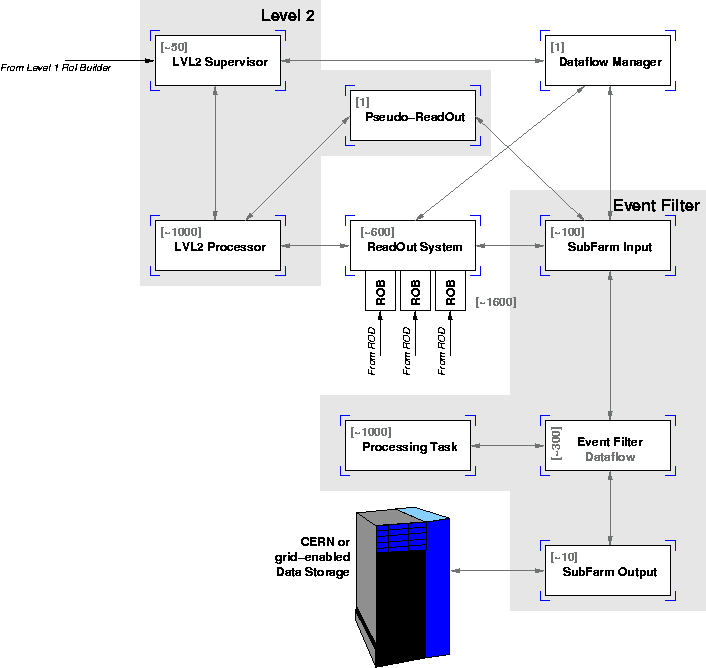
\includegraphics[scale=0.65]{dfbasic}
\end{center}
\caption{Os componentes do DF e suas interconexões.}
\label{fig:dfbasic}
\end{figure}

A seqüência de funcionamento se dá da seguinte forma: o Supervisor do LVL2
(\gls{glos:l2sv}) recebe uma mensagem do RoIB do LVL1 indicando a ocorrência
de um evento interessante e aprovado por este nível. Somente há um RoIB no
sistema, que envia para o primeiro Supervisor do LVL2 disponível a mensagem
sobre o evento. Cada Supervisor mantém um conjunto de Unidades de
Processamento do LVL2 (do inglês \eng{LVL2 Processing Unit}, \gls{glos:l2pu})
em sua lista de nós supervisionados. Logicamente atrelado a cada L2PU há uma
fila de eventos que foram recentemente alocados para processamento. O L2SV
localiza a L2PU com menos eventos atribuídos e envia a mensagem do LVL1 para
este processador.

A L2PU decodifica a mensagem enviada pelo L2SV e analisa as regiões do detetor
de que precisará para processar o evento. O tamanho e a quantidade de dados de
que a L2PU necessitará para processar o evento dependem dos algoritmos que são
lá executados e, portanto, este processador tem livre arbítrio na quantidade e
qualidade dos dados que irá requisitar. Para coletar os dados, a L2PU computa
o número e a localização dos ROB's que são necessários, e encaminha um pedido
de dados prontamente ao Sistema de Leitura do Detetor (do inglês, \idxeng{Read
Out System}, \gls{glos:ros}). Os ROS's afetados respondem com os dados dos ROB's
relevantes e, desta forma a L2PU poderá classificar o evento. Após algum
intervalo de tempo necessário à análise da Física do evento, a L2PU responde
ao L2SV com um valor binário, indicando rejeição ou aceitação do evento. Se o
evento for aceito, a L2PU também envia um diagnóstico do que foi encontrado no
evento para dentro de um pseudo-ROS (\gls{glos:pros}), que permitirá a
anexação desta informação ao evento final.

A segunda parte do processamento do evento nos altos níveis de filtragem é
iniciada por uma mensagem do L2SV ao Gerente do Fluxo de Dados (do inglês,
\eng{Dataflow Manager}, \gls{glos:dfm}), indicando o destino de todos os eventos até
então aprovados pelo LVL1. No caso de um determinado evento ser
desconsiderado, o DFM envia uma mensagem para o ROS indicando que este deverá
apagá-lo dos \eng{buffers}, ou em caso contrário enviará uma mensagem
indicando ao processador de construção de eventos (\eng{SubFarm Input},
\gls{glos:sfi}) que deverá coletar os fragmentos do evento. O SFI então envia
mensagens a cada um dos ROS's no sistema e requer todas as informações
disponíveis para o evento de interesse. O objetivo do SFI é aglutinar todas as
partes do evento em um único espaço de memória, liberando as partes anteriores
do sistema do encargo do gerenciamento deste mesmo espaço.

Uma vez construído, o evento é guardado em uma pilha lógica dentro do SFI que
aguarda um pedido de um Gerente do Filtro de Eventos (do inglês, \eng{Event
Filter Dataflow Manager}, \gls{glos:efd}), indicando que está disponível para
processar mais um evento. Este evento é transferido integralmente para o EFD
neste momento. O EFD, de forma análoga ao L2SV, verificará a Unidade de
Processamento (\eng{Processing Task}, \gls{glos:pt}) disponível e a alocará
para tratar as informações deste evento. Neste momento, todo o evento (com
seus dados) é disponibilizado à PT, que poderá levar mais tempo processando o
evento que sua análoga no LVL2, dada a taxa reduzida de eventos
remanescentes. Se aprovado, o evento é encaminhado a um processador de saída
(\eng{SubFarm Output}, \gls{glos:sfo}), que coopera com o sistema de gravação
de dados na disponibilização dos eventos colhidos pelo DAQ. O sistema também é
equipado com dispositivos que garantem o funcionamento de cada componente na
falha de outros ou quando algum nó ou nós começam a responder mais lentamente
provocando congestionamentos. Para funcionar plenamente, o \eng{Dataflow} está
montado sobre as bases do Sistema \eng{Online}, que provê as ferramentas de
controle e configuração necessárias para operar uma cadeia de aquisição
completa.

\subsubsection{Ferramentas do \eng{dataflow}}
\label{sec:dftools}

Para se projetar um conjunto de aplicações que funcionem coerentemente é
necessário partir de uma base funcional comum. Desta forma, optou-se pelo
projeto e construção de um conjunto de ferramentas que fornecem uma base para
o desenvolvimento das aplicações do DF. Estas ferramentas incluem:

\begin{itemize}
\item Ferramentas para isolamento do Sistema Operacional: reúnem um
conjunto de bibliotecas que executam funções primárias como a criação de
tarefas (para ambientes multi-tarefa), relógios e primitivas como filas
protegidas. Esta camada de funções também isola, dentro do possível, variações
no sistema operacional de alterações no código das aplicações do DF;

\item Ferramentas para troca de mensagem: provêem uma interface simples para a
troca de mensagens entre aplicações. Os canais de comunicação são
configuráveis, permitindo o tráfego (transparente) de dados diretamente sobre
pacotes \eng{ethernet}, UDP ou TCP. Este pacote também engloba ferramentas
para a codificação e decodificação dos dados provenientes dos detetores.

\item Ferramentas para configuração: provêem interfaces para a configuração dos
aplicativos utilizando o Sistema \eng{Online};

\item Ferramentas para controle e relatório de erros: permitem o envio de
mensagens de erro e depuração para os nós de controle da cadeia de
aquisição. Este conjunto de ferramentas também inclui os aplicativos, nos
moldes da máquina de estados apresentada na Figura~\ref{fig:online-fsm}.
\end{itemize}

Para aumentar a qualidade dos programas desenvolvidos e a manutenção a longo
prazo (o experimento deve operar por 10 anos ou mais), optou-se por utilizar
técnicas de orientação a objetos (OO) aplicadas sobre C++. Alguns problemas,
e.g. ineficiência da utilização dos \eng{containers}-padrão da biblioteca
padrão (\eng{Standard Template Libraries}, STL) C++ em ambientes multi-tarefa,
advieram desta decisão \cite{aa:chep-2003}. De fato, a alocação de memória
implementada pelos compiladores da linha GCC \cite{web:gcc, web:gcc-stl} visa
a otimização da alocação de memória por processo enquanto em ambientes
multi-tarefas (do inglês \eng{multi-threading}) é necessária a utilização de
pilhas separadas para cada tarefa. A solução neste caso foi a adoção de
alocadores mais eficientes para este propósito, que não fazem parte do padrão
C++.

\subsection{Fluxo de dados e a arquitetura no LVL2}
\label{sec:lvl2arch}

Especificamente para este trabalho, a arquitetura e o funcionamento do segundo
nível de filtragem do experimento são de especial atenção. É possível observar
na Figura~\ref{fig:lvl2arch} um esquema da troca de mensagens das aplicações
no LVL2, como anteriormente indicado na área acinzentada da
Figura~\ref{fig:dfbasic}. Nesta figura, as linhas tracejadas indicam mensagens
de controle do sistema e as linhas cheias, as mensagens que carregam dados do
detetor ou resultados da operação de filtragem. Inicialmente, o Supervisor do
LVL2 recebe uma mensagem contendo as informações das RoI encontradas pelo
LVL1. As RoI's equivalem a objetos encontrados, seja nos detetores de múons ou
nos calorímetros, com energia mínima para a ativação dos subseqüentes níveis
de filtragem. Esta mensagem é chamada de Resultado do LVL1, e abreviadamente
de ``L1R''. A mensagem que chega ao L2SV representa, portanto, uma avaliação
do evento com uma qualidade equivalente à visibilidade que o LVL1 tem do
detetor. Para continuar com a avaliação do evento, o L2SV alocará uma L2PU que
esteja sob sua guarda para processá-lo.

\begin{figure}
\begin{center}
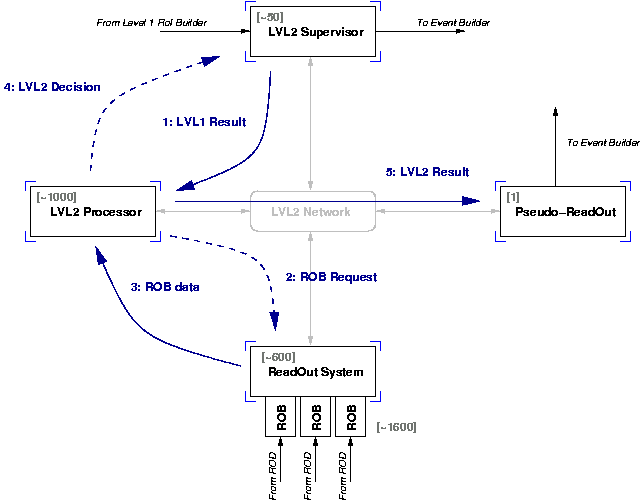
\includegraphics[scale=0.7]{lvl2arch}
\end{center}
\caption{A ordem das mensagens trocadas pelas aplicações do LVL2.}
\label{fig:lvl2arch}
\end{figure}

A L2PU processa eventos por RoI. Para cada RoI encontrada em um resultado do
LVL1, a L2PU requisitará os dados ao redor do objeto e avaliará novamente o
objeto, levando em conta a máxima granularidade do detetor ao redor daquele
ponto. Se o objeto encontrado pelo LVL1 tiver sido achado através de sua
interação com o calorímetro, o LVL2 requisitará inicialmente os dados deste
sub-detetor. Caso o objeto tenha sido encontrado nos detetores de múons, o
processamento começará a partir deste sub-sistema. O processamento de cada
evento na L2PU se dá de forma seqüencial. Para cada RoI destacada pelo LVL1 é
feita uma confirmação da análise do LVL1 contando com a melhor precisão
disponível para os dados avaliados e possíveis validações cruzadas, levando-se
em conta dados dos detetores internos. Se a RoI for rejeitada, o processamento
é abortado e imediatamente uma mensagem de controle é enviada ao L2SV
indicando um evento inválido. Caso as diversas etapas de processamento se
confirmem ao longo da análise do evento, a resposta ao L2SV é atrasada até que
o evento seja confirmado em última instância ou rejeitado no meio do
processamento. Nota-se aqui que eventos interessantes terão maior tempo de
processamento que eventos ordinários, já que os últimos serão rejeitados assim
que possível, enquanto que os primeiros terão que ser aprovados por todos os
critérios de processamento no LVL2. O processamento como um todo continua
requisitando dados, conforme a necessidade, aos diversos ROS's, até que a L2PU
possa concluir, com baixíssima probabilidade de erro, se o evento deve ser
aprovado ou rejeitado.

O L2SV opera de forma indiferente à rejeição ou aceitação do evento por um
Processador do LVL2, já que repassará todas as mensagens, possivelmente
agrupadas para melhorar o desempenho da comunicação de pacotes, ao DFM. Por
outro lado, a cadeia de processamento para a L2PU se dá de forma ligeiramente
diferente se tiver um evento confirmado. Caso o evento seja rejeitado, somente
uma mensagem de controle é enviada ao L2SV. De outra forma a L2PU deverá,
antes da mensagem de controle, enviar um extrato completo das operações
executadas a um \eng{buffer} indicado na Figura~\ref{fig:lvl2arch} por
\eng{Pseudo ReadOut}, PROS. Este único processador do sistema opera como um ROS,
porém, ao invés de coletar dados de ROB's, armazena os resultados
(diagnósticos) de eventos bem-sucedidos do LVL2, servindo estes resultados a
um SFI quando o evento é construído. É desta forma que o resultado das
operações do LVL2 poderá chegar ao Filtro de Eventos. O PROS é uma aplicação
bastante simples que fornece 2 interfaces (lógicas) de rede. A primeira coleta
os dados de todas as L2PU's do sistema e a segunda responde a requisições dos
SFI's que desejam construir os eventos aprovados.

Após enviar o resultado das operações do LVL2 (L2R) ao PROS, a L2PU poderá
enviar a mensagem de aceitação ao L2SV. Desta forma garante-se que a
construção do evento operará corretamente, uma vez que o PROS não receberá um
pedido para enviar o L2R antes de o ter recebido. O processamento prosseguirá
desta forma por períodos que durarão até 10 horas e, portanto, erros de
programação e, principalmente, vazamentos de memória são proibitivos neste
árduo ambiente.

O orçamento do sistema é otimizado para canalizar a maior quantidade de
recursos possível em poder de classificação de eventos. Portanto, a relação
entre o número de L2PU's e os demais nós de processamento deve ser tão grande
quanto possível. Atualmente estima-se que serão necessários cerca de 1.000
processadores (operando como L2PU's) para suportar a taxa de entrada de
eventos de 100 kHz. Dado o paralelismo inerente ao processo, cada L2PU deverá
processar um evento em não mais do que 10 milissegundos, i.e., cada um poderá
suportar uma taxa de 100 Hz.

\subsubsection{Arquitetura da L2PU}
\label{sec:l2puarch}
A arquitetura da L2PU pode ser melhor descrita através da
Figura~\ref{fig:l2puarch}, onde é possível observar três componentes
primários:

\begin{itemize}
\item Tarefa de Entrada (\eng{input thread}): Centraliza o recebimento de dados
dentro da L2PU. Cada tipo de mensagem recebida está associada a um manuseador
(\eng{handler}) distinto que especifica o destino a ser dado à mensagem
recebida. Por exemplo, mensagens do L2SV indicando resultados do LVL1 são
encaminhadas para uma pilha protegida;

\item Pilha Protegida: Controla o acesso concorrente das tarefas processadoras
(\eng{worker threads}) aos resultados do LVL1 depositados na L2PU;

\item Tarefas Processadoras: É onde o processamento (seqüencial) de cada
evento é feito. Cada tarefa possui um Coletor de Dados que é responsável pela
comunicação com os ROS's disponíveis para reunir os dados necessários a cada
passo do processamento de um evento.
\end{itemize}

\begin{figure}
\begin{center}
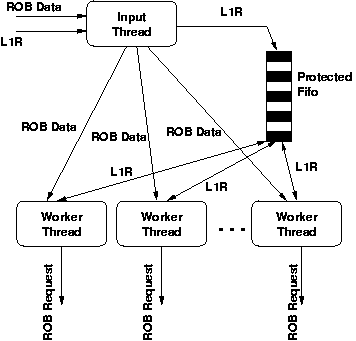
\includegraphics[scale=0.8]{l2puarch}
\end{center}
\caption{A arquitetura da L2PU.}
\label{fig:l2puarch}
\end{figure}

Ao receber um L1R do Supervisor, a tarefa de entrada irá colocá-lo numa pilha
tipo FIFO (\eng{First In First Out}) protegida ao acesso concorrente da cada
uma das tarefas processadoras. As tarefas concorrem na aquisição de um L1R
para iniciar o processamento e, caso tenham sucesso, saem do modo de espera,
onde praticamente não consomem a CPU do sistema hospedeiro, e iniciam a
discriminação do evento. Para isso, requisitam dados aos ROS's disponíveis que
enviarão, dentro de suas possibilidades, os fragmentos da RoI equivalentes ao
subdetetor de interesse. É possível que determinados ROS's não consigam
responder ao tempo máximo de espera da L2PU e, neste caso, o evento deve ser
processado com dados faltantes. Há outras possibilidades que podem comprometer
a integridade dos dados que serão finalmente manipulados na L2PU, já que a
cadeia de aquisição, passando pela eletrônica de aquisição acoplada ao
detetor, os ROB's e finalmente os ROS's, podem apresentar inúmeros tipos de
falhas que resultarão na perda dos dados analisados pela L2PU, total ou
parcialmente. Os algoritmos de discriminação devem estar preparados para estas
anomalias de funcionamento, e devem ser construídos para consumir o mínimo
possível de dados, já que, além da maior probabilidade de falhas, mais dados
também significam maior banda passante necessária à rede que interliga estes
dois nós de processamento.

Os fragmentos de RoI (e também do detetor) que são carregados pela L2PU são
armazenados e transmitidos em um formato particular, e uma biblioteca de
codificação e decodificação \cite{aa:ef-urd, aa:ef-ooad} está disponível para
este propósito. Os dados não são somente decodificados, mas também
re-arranjados e calibrados antes do uso, o que pode consumir grande parte do
tempo de processamento (10 ms) no LVL2.

O L2R juntamente com a decisão do LVL2 são enviados diretamente das tarefas
processadoras ao L2SV e ao PROS sem a intervenção de outros componentes dentro
da L2PU.

\subsubsection{Parâmetros de \eng{hardware} do DAQ}

A escolha da tecnologia de processamento, tal qual aquela empregada para a
rede de interconexão destes nós, é um parâmetro vital para viabilização do
Sistema de Aquisição de Dados do ATLAS. Diversos aspectos devem ser
considerados:

\begin{itemize}
\item Econômico: Deve-se maximizar os recursos disponíveis. Desta forma,
deseja-se despender o mínimo necessário em recursos para a compra de
equipamento. Por ``mínimo necessário'' entende-se o mínimo necessário para
operar, de forma cômoda, o experimento por 10 anos;

\item Operacionais: O equipamento deve ter sua operabilidade maximizada. Deve
ser relativamente fácil repor componentes ou realizar atualizações que não
impliquem a reposição de toda a cadeia de aquisição. A manutenção e operação
dos programas deve ser acessível a novos usuários.
\end{itemize}

Por estas razões decidiu-se pela utilização de equipamentos disponíveis no
mercado de comodidades atual: PC's operando sobre redes padrão (\eng{gigabit}
ou 10-\eng{gigabit}) ethernet. O sistema operacional escolhido foi Linux. A
razão desta escolha se deve a estabilidade do sistema em operação contínua e a
confiabilidade dos módulos para conexão em rede. A utilização de um sistema
operacional aberto, gratuitamente distribuído, também facilita o
desenvolvimento de \eng{drivers} especializados para atividades específicas.

Para maximizar a operabilidade e diminuir o custo, pretende-se adquirir
máquinas com dois ou quatro núcleos de processamento com memória compartilhada
(arquitetura \gls{glos:smp}, do inglês \eng{Symmetric Multi-Processor}). Esta
arquitetura apresenta várias vantagens:

\begin{itemize}
\item Para cada 2 ou 4 processadores, somente 1 disco e 2 interfaces de rede
serão necessárias\footnote{Uma das interfaces de rede é alocada para sinais e
dados de controle enquanto a outra funciona exclusivamente para o tráfego de
dados do detetor. Nesta configuração, somente uma das duas interfaces de rede
necessita de uma banda passante maior, a interface por onde trafegarão os
dados obtidos no detetor.}. Desta forma, não há somente economia de espaço e
dinheiro, mas também no tamanho da rede final que será projetada;

\item Há também economia de energia durante a operação e, principalmente,
durante o momento de ligar as máquinas. A conexão concomitante de 2.500 discos
rígidos pode acarretar problemas de super-aquecimento do \eng{cluster} e
quedas de tensão em outros pontos do sistema.
\end{itemize}

A arquitetura da L2PU, apresentada na Seção~\ref{sec:l2puarch}, deriva desta
escolha do equipamento. Uma vez que somente uma das interfaces estará
disponível para o tráfego de dados, a utilização de mais tarefas para esta
atividade torna-se desnecessária. O número de tarefas processadoras, no
entanto, deve ser otimizado para que o sistema atinja o seu desempenho máximo.

\subsection{Análise funcional do fluxo de dados no LVL2}
\label{sec:lvl2work}

Para avaliar a correta operação dos diversos processos que compõem o LVL2, é
necessário operar os diversos componentes em uma bancada de teste (do inglês
\eng{testbed}). Por razões econômicas, o sistema em sua escala de produção
(cerca de 2.500 nós de processamentos) somente estará disponível em uma data
próxima ao início de operação do detetor. Por outro lado, a transferência na
data de compra também possibilita a aquisição de processadores mais potentes
pelo mesmo custo. Desta forma, as \eng{testbeds} disponíveis para teste, ainda
que representando o estado da arte dos equipamentos escolhidos, são de tamanho
reduzido, se comparadas ao sistema final.

De forma a qualificar a avaliação de cada componente, faz-se necessário criar
condições de operação que satisfaçam o modelo de operação final. Com relação
ao LVL2, muitos modelos foram explorados \cite{aa:tns-2004} ao longo de 2 anos
de testes. Estes modelos e a verificação do funcionamento coerente desta parte
do sistema de aquisição encontram-se sintetizados nesta seção \cite{hlt-tdr}.

Como será detalhado mais adiante, na Seção~\ref{sec:hlt}, os módulos que
executam a análise da Física de interesse são carregados dinamicamente na
L2PU, através de parâmetros de configuração disponíveis ao operador do
experimento. Esta estratégia permite que o sistema de fluxo de dados seja
testado independentemente dos algoritmos de filtragem, paralelizando o
desenvolvimento \cite{aa:tns-2004-2} e reduzindo significativamente as
possibilidades de falha devido a componentes que não sejam relevantes para a
natureza dos testes. Para os processos descritos nesta seção, foram utilizados
emuladores dos componentes de discriminação, que podem simular a aquisição de
dados de RoI's e até o tempo de processamento entre tomadas de dados,
possivelmente em múltiplos passos. Este bloco emulador é sintonizado para
caracterizar os parâmetros normais de operação do LVL2.

\subsubsection{Parâmetros críticos do sistema de leitura}

Um dos parâmetros que se deseja investigar é a capacidade da L2PU de coletar
dados do sistema de leitura, neste caso representado pelos diversos
ROS's. Como colocado anteriormente, ao processar um resultado do L1R, a L2PU
começa por confirmar o resultado encontrado no nível precedente, utilizando,
para isso, a granularidade máxima do detetor ao redor da RoI. O tamanho da RoI
dependerá diretamente dos valores discriminantes que devem ser
encontrados. Algumas modalidades de algoritmos podem requerer mais dados e,
portanto, aumentar significativamente o tráfego de dados na rede. Algoritmos
mais eficientes tenderão a consumir dados em pequenas parcelas, minimizando o
tempo de rejeição necessário para cada evento do ruído de fundo. É possível,
em todos os casos, adquirir pequenas parcelas de dados inicialmente e aumentar
o campo de atuação do algoritmo à medida que o evento não é rejeitado. Por
outro lado, também é possível compartimentalizar a aquisição de dados por
sub-detetores. Cada estágio do processamento seqüencial do evento adquirirá,
neste modelo, dados de diferentes camadas do ATLAS. A solução ótima está
provavelmente na utilização das duas técnicas, ou seja, o consumo parcelado de
dados para cada sub-detetor com rejeição assim que possível. Uma rejeição
rápida garante mais tempo para o processamento de eventos realmente
interessantes e minimiza o tráfego de rede.

Cada L2PU, como visto anteriormente, mantém uma fila tipo FIFO com eventos
alocados pelo Supervisor do LVL2. A maximização do tempo de processamento
disponível depende, portanto, da não-escassez de eventos nesta fila, uma vez
que com a fila vazia, uma ou mais das tarefas processadoras serão
bloqueadas. Desta forma, o L2SV é sintonizado cuidadosamente para que esta
situação nunca ocorra.

Ainda que o número e o tamanho médio das RoI's dependam da Física a ser
avaliada, o fator de concentração de ROB's (o número de ROB's que deve ser
lido de cada ROS) é um parâmetro que deve ser otimizado. Variações de
desempenho nesta área indicam melhores geometrias para a interconexão do
sistema de leitura do detetor e a rede que liga o LVL2. Por outro lado, o
número ótimo de tarefas processadoras operando dentro de cada L2PU dependerá
do tempo-morto despendido durante a aquisição de dados e do número de
processadores disponíveis em cada máquina. Em máquinas com dois núcleos de
processamento, por exemplo, o número ótimo de tarefas processadoras deve estar
entre 3 e 4, já que o uso de um número menor deste tipo de tarefas implicará
na sub-utilização do poder de processamento de cada nó.

Medidas foram realizadas no CERN, variando-se parâmetros críticos para o
desempenho da coleta de dados para RoI's. A contribuição gerada pela coleta
de dados para uma RoI, ao tempo de processamento de uma L2PU em função do
tamanho da RoI e o número de ROS's na qual a RoI está distribuída, é mostrada
na Figura~\ref{fig:tns-4fig}. Estes testes foram executados em uma bancada com
apenas um L2SV, doze ROS's e uma L2PU. Todos os nós nesta bancada de teste são
PC's com dois núcleos tipo Intel/Xeon's de 2,2 GHz e 1 \eng{gigabyte} de
memória RAM, interconectados por uma chave padrão \eng{gigabit} ethernet. Na
figura, no eixo vertical é possível observar a taxa de processamento inversa
de um L2SV com uma única L2PU sob seu controle. Este parâmetro representa o
tempo médio que cada evento levou para ser inteiramente processado pelo LVL2,
ou seja:

\begin{figure}
\begin{center}
\includegraphics{tns/4fig}
\end{center}
\caption{Desempenho da coleta de dados de RoI para várias combinações de
tamanhos de RoI (em bytes) e tarefas processadoras. Extraída de
\cite{aa:tns-2004}.}
\label{fig:tns-4fig}
\end{figure}

\begin{enumerate}
\item O tempo de envio do resultado do LVL1 para o L2PU;
\item A aquisição do resultado pela tarefa processadora;
\item O mapeamento da RoI nos ROB's de interesse;
\item A aquisição dos dados dos ROS's;
\item A resposta para o L2SV, indicando aceitação ou rejeição.
\end{enumerate}

Neste caso, o tempo de processamento para os dados foi ajustado para zero. A
resposta da L2PU ao L2SV é sempre negativa (para evitar o envio do L2R ao
PROS). 

No eixo horizontal da Figura~\ref{fig:tns-4fig}, é possível observar o número
de ROS's que contribuíram para os dados na RoI. O conjunto de medidas
apresentado nesta figura corresponde a valores de tamanhos de RoI realísticos
para dados partindo da seção e.m. do calorímetro, representando este o pior
dos casos. Para este sub-detetor, estima-se que a RoI para os dados de todas
as três camadas do detetor encontre-se espalhada por 13 a 16 ROB's e tenha um
tamanho total, em média, de 16 quilobytes. É possível notar, através
deste gráfico, que o tempo de coleta de dados contribui, no pior dos casos,
com apenas 10\% do tempo de processamento médio estimado para cada evento no
LVL2 (10 milissegundos).

Podemos também notar que o aumento no número de tarefas processadoras de 1
para 4 modifica significativamente o perfil do tempo-morto gasto na aquisição
de dados, já que não haverá esperas espontâneas no sistema, como colocado
anteriormente neste texto. No caso de 4 tarefas processadoras, o tempo de
coleta de dados está na ordem de 600 microssegundos. Podemos também observar
que com maior distribuição de dados no sistema (mais ROS's), o tempo de
coleta de dados de uma RoI aumentará numa relação aproximadamente linear, o
que casa bastante bem com o modelo OO apresentado. A minimização do número de
ROS's é portanto desejável para um tempo-morto menor.

Na Figura~\ref{fig:tns-5fig} observa-se o desempenho de uma única L2PU contra
a taxa de operação de um L2SV invertida para um número variável de tarefas
processadoras. Neste teste o tamanho da RoI está fixo em 16 quilobytes. As
diferentes curvas representam a mesma RoI sendo coletada de 2, 4, 8 ou 16
ROS's. Por exemplo, a curva superior representa os resultados para coletar uma
RoI de 16 quilobytes de 16 ROS's (1 quilobyte por ROS). O resultado
indica que o número ótimo de tarefas processadoras para esta bancada de testes
(sistemas com dois núcleos) é de, aproximadamente, três e é independente
do número de ROS's dos quais os dados da RoI estão sendo coletados. Ademais,
os resultados mostram que, para as condições deste teste, e para 3 tarefas
processadoras, a coleta de dados contribui com menos de 10
\% do tempo de processamento médio esperado no LVL2 de 10 ms. Isto concorda
com o estudo anterior.

\begin{figure}
\begin{center}
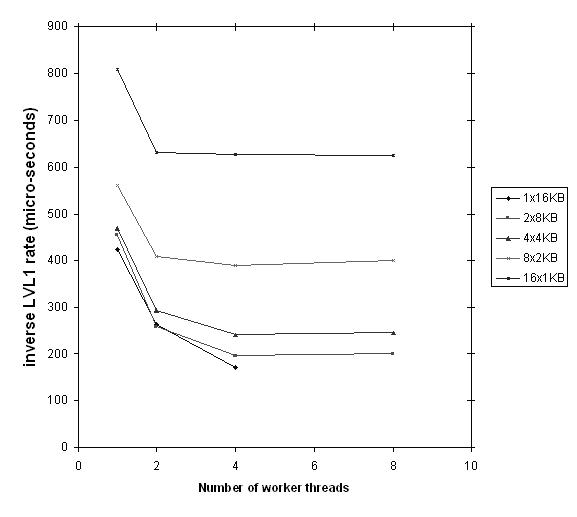
\includegraphics[scale=0.9]{tns/5fig}
\end{center}
\caption{A taxa inversa em um L2SV para uma única L2PU funcionando com
diferentes números de tarefas processadoras. Extraída de
\cite{aa:tns-2004}.}
\label{fig:tns-5fig}
\end{figure}

\subsubsection{Escalabilidade do LVL2}

Os testes apresentados até agora mostraram a taxa com a qual uma L2PU pode
coletar dados, se não estiver equipada com algoritmos de discriminação de
eventos. O desempenho atingido depende do tamanho da RoI, o fator de
concentração de ROB's por ROS's e do número de tarefas processadoras
disponível neste processador. Para o sistema de aquisição como um todo, no
entanto, é também necessário demonstrar que, quando muitas L2PU's estão
coletando dados ao mesmo tempo do mesmo conjunto de ROS's, o desempenho da
coleta de RoI's não degrada de forma inaceitável.

Para este teste, L2PU's não equipadas de algoritmos de filtragem reais foram
usadas novamente e, por esta razão, deve ser notado que a taxa de envio de
mensagens de cada um destes nós estará operando num patamar bastante acima do
que o sistema real necessitará. Para estes testes, cada L2PU estará gerando 10
vezes mais tráfego que o esperado no sistema final. De forma análoga e
aditiva, o número de ROS's do sistema também não é ideal, devido à baixa
disponibilidade de equipamento para testes. É, portanto, necessário garantir
que a taxa de requisições de dados para cada ROS não exceda um valor limite
que mascararia quaisquer resultados obtidos.

Estes testes foram executados em uma bancada com três L2SV's, quatro ROS's e
até onze L2PU's. Todos os nós nesta bancada de teste são PC's, na mesma
configuração de antes, interconectados por uma chave padrão \eng{gigabit}
ethernet. Para este teste, cada ROS foi configurado para emular 12 conexões
com ROB's, gerando um total de 48 ROB's para este teste. Para cada requisição,
a L2PU escolhe um dos 48 ROB's aleatoriamente e um número de ROB's com
numeração consecutiva. Por exemplo, no caso em que cada RoI consista de 6
ROB's, a L2PU seleciona o primeiro aleatoriamente e completa o pedido com
outros 5 ROB's cuja numeração sucede o primeiro ROB. Se o último ROB fosse
selecionado, o algoritmo voltaria ao primeiro ROB disponível
(\eng{wrap-around}).

A Figura~\ref{fig:tns-6fig} traz os resultados sintetizados desta
bancada. Nesta figura é possível observar a taxa de eventos média tratados em
cada L2PU em função do número de L2PU's usadas no teste para uma RoI
distribuída por 1, 6 ou 24 ROB's (com cerca de 1,5 quilobyte por
ROB). Observa-se na figura que a taxa por L2PU diminui quando o número de
L2PU's aumenta, por aproximadamente 20\% para 1 ROB por RoI e aproximadamente
40\% para 24 ROB's por RoI. Entretanto, com 11 L2PU's configurados na bancada,
a taxa de requisições por ROS é de 17 kHz para 1 ROB por RoI e de 8 kHz para
24 ROB's por RoI. Estas duas situações representam uma sobrecarga jamais
atingível no sistema final. A taxa total de requisições de dados de RoI nesta
pequena bancada de testes é de 70 kHz e 11 kHz para os dois números de ROB's
por RoI indicados.

\begin{figure}
\begin{center}
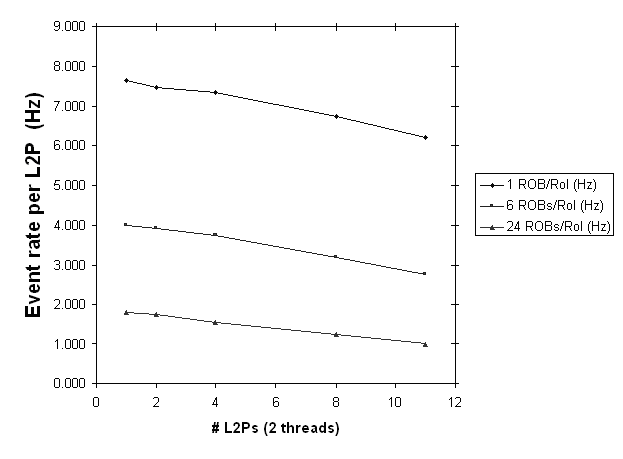
\includegraphics[scale=0.9]{tns/6fig}
\end{center}
\caption{A taxa de eventos média para cada L2PU em função do número de
L2PU's no sistema para diferentes números de ROB's por RoI. Cada ROB contribui
com um montante igual dos dados da RoI. Extraída de
\cite{aa:tns-2004}.}
\label{fig:tns-6fig}
\end{figure}

Na Figura~\ref{fig:tns-scale-burn} é possível observar os resultados de uma
bancada de testes equivalente contendo 1, 2, 4 e 8 L2PU's. Porém, desta vez,
ajustou-se o tempo de processamento emulado para cada evento em 1
milissegundo. Isto representa apenas a décima parte do esperado no sistema
final. Nesta figura, é possível observar um bom escalonamento do
sistema. Dadas as extremas condições recriadas nestas bancadas, é razoável
assumir que a escalabilidade do sistema final se mostrará aceitável às
condições do DAQ.

\begin{figure}
\begin{center}
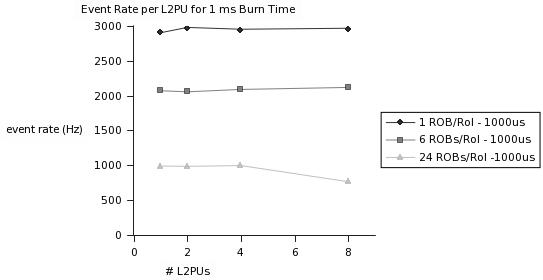
\includegraphics[scale=0.7]{tns/scale-1msburn}
\end{center}
\caption{A taxa de eventos média para cada L2PU em função do número de L2PU's
no sistema. O tempo de processamento emulado para cada evento é de 1
ms. Extraída de \cite{aa:tns-2004}.}
\label{fig:tns-scale-burn} 
\end{figure}

Observa-se na Figura~\ref{fig:tns-7fig} a taxa sustentada por um L2SV em
função do número de L2PU's sob seu controle. Nesta bancada, o nó de
processamento rodando o L2SV está conectado através de uma chave \eng{gigabit}
ethernet, com um número de outras máquinas rodando o código da L2PU sem
algoritmos de discriminação carregados e sem coletar dados dos ROS's. Este é
portanto um teste extremo, visto que as L2PU's vão responder o mais rápido
possível a cada requisição de processamento de eventos feita pelo L2SV. Como
pode ser visto pela figura, um único L2SV pode sustentar a taxa de 32~kHz
enquanto distribuindo L1R's para apenas uma das L2PU's sob seu controle, e a
dependência no número de L2PU's está na ordem de 1\%. Desta forma, tomando-se
como ponto de partida a implementação do sistema de fluxo de dados e as
máquinas, cerca de 10 L2SV's seriam capazes de suprir a taxa de entrada do
LVL2. Há, todavia, outros fatores não considerados nesta suposição, tais como
robustez e a conexão com o DFM, que certamente penaliza a taxa de
processamento. Levando-se todos os pontos em questão, parece ser razoável
contar com a presença de 30 a 50 L2SV's no sistema final.

\begin{figure}
\begin{center}
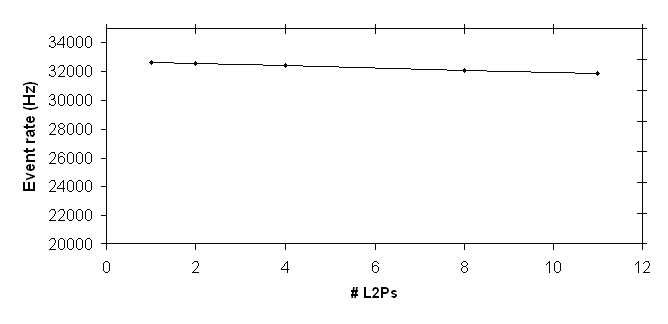
\includegraphics[scale=0.8]{tns/7fig}
\end{center}
\caption{A taxa sustentada por L2SV com o aumento de L2PU's no
sistema. Extraída de \cite{aa:tns-2004}.}
\label{fig:tns-7fig}
\end{figure}

Os testes aqui descritos descrevem e comprovam o funcionamento da
infraestrutura que permite o acoplamento dos algoritmos que executam a
discriminação dos eventos lidos pelo detetor ATLAS. A eficiência destes mesmos
algoritmos é de extrema importância para o desempenho final do sistema de
filtragem. Um conjunto de procedimentos ineficaz e lento será mais oneroso
economicamente e também tecnicamente, já que a qualidade dos eventos
finalmente aprovados se torna duvidosa.

\subsection{Altos níveis de filtragem e seus algoritmos}
\label{sec:hlt}

A infraestrutura de seleção de eventos dos Altos Níveis de Filtragem constitui
o ambiente de processamento para os algoritmos de discriminação do DAQ. Esta
infraestrutura é comum ao LVL2 e ao EF, e é composta de 4 partes distintas. O
Gerente do HLT (ou, do inglês, \eng{Steering}) agenda os algoritmos do HLT
correspondentes ao tipo de evento que está sendo analisado. Informações sobre
quantidades físicas específicas a um evento são trocadas através de
componentes do Modelo de Dados do Evento (do inglês \eng{Event Data Model},
\gls{glos:edm}). Durante o processamento, os dados gerados são guardados e
acessados através de um Gerente de Dados (do inglês, \eng{Data Manager},
\gls{glos:dm}). Isto permite transparência às escolhas de plataforma de
armazenamento e tecnologia utilizadas para executar as operações de
filtragem. Os algoritmos do HLT propriamente ditos reconstroem quantidades
relativas aos eventos ou confirmam hipóteses através de quantidades
previamente calculadas. A Figura~\ref{fig:hlt-arch} ilustra o relacionamento
entre estes macrossistemas do HLT com alguns exemplos de classes
representativas.

\begin{figure}
\begin{center}
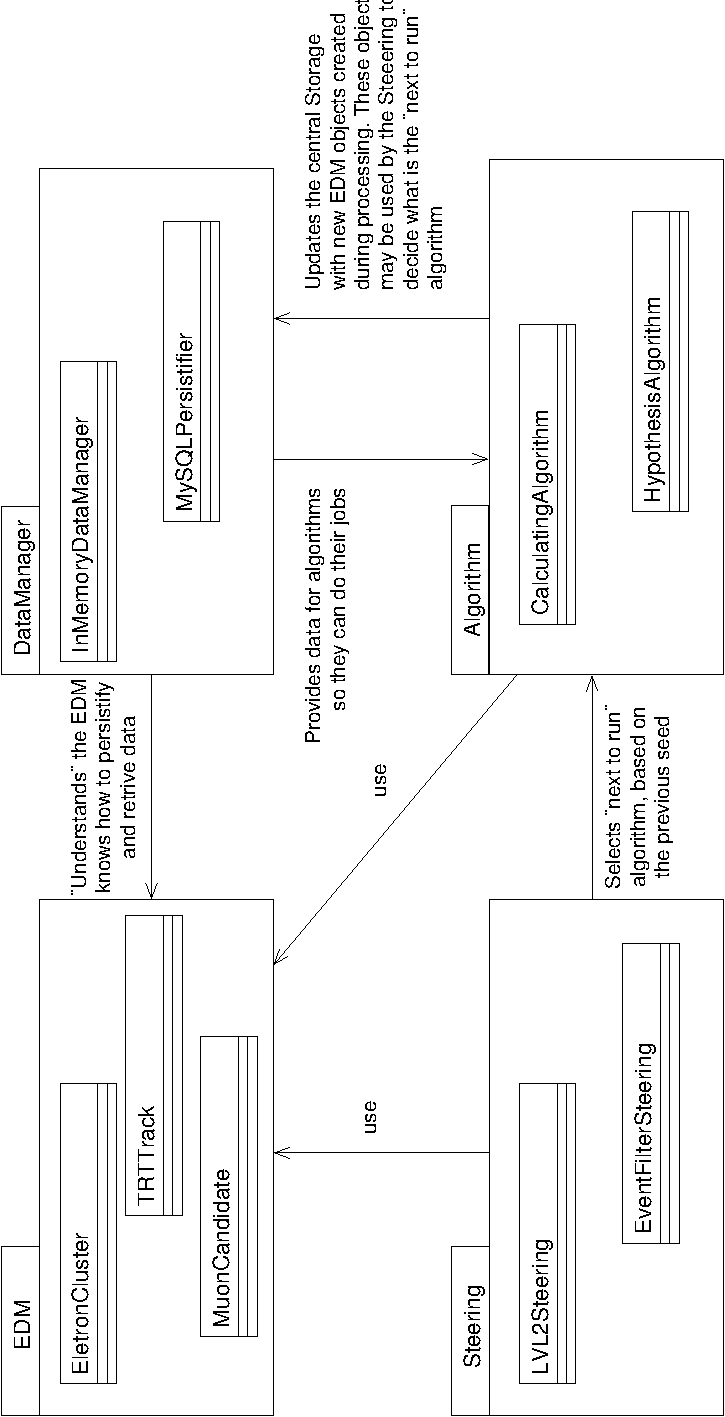
\includegraphics[scale=0.8,angle=90]{hlt-arch}
\end{center}
\caption[Relação entre os macrossistemas do HLT.]{Relação entre os
macrossistemas do HLT. Extraído de \cite{hlt-tdr}.}
\label{fig:hlt-arch}
\end{figure}

Uma vez que o propósito do \eng{software} de discriminação de eventos do HLT é
a seleção de eventos, ele deve executar de maneira eficiente e confiável no
ambiente do DAQ/Fluxo de Dados. Os componentes críticos para a seleção devem
ser portados ao ambiente \eng{offline} para seu desenvolvimento e
teste. Provendo um conjunto básico de interfaces para ambos os cenários, o HLT
garante a consistência para o desenvolvimento do sistema de
filtragem. Ademais, alguns estudos \cite{jb:e-gamma} mostram que um grande
custo computacional pode ser economizado com a otimização global do sistema de
filtragem quanto à ordem e a qualidade dos algoritmos executados. A existência
de uma infraestrutura comum também facilita este tipo de estudo.

Uma vez que o Filtro de Eventos provê um ambiente de computação praticamente
igual ao ambiente \eng{offline}, o conjunto de rotinas do HLT é naturalmente
baseado no ambiente de análise \eng{offline}, Athena, que por sua vez é
baseado na infraestrutura de análise física Gaudi \cite{athena:home-page,
athena:devel-guide}. Esta estratégia permite a re-utilização do Gerente de
Dados, do EDM, da descrição dos detetores e de muitos algoritmos que já se
encontram desenvolvidos por esta comunidade. Apenas o Gerente do HLT
(\eng{Steering}) e determinados algoritmos restam como desenvolvimentos
específicos a este sub-sistema. No caso específico do LVL2, um enfoque similar
torna-se mais complexo, já que o processo de seleção ocorre em múltiplas
tarefas concorrentes às unidades de processamento disponíveis e restrições
mais severas tornam-se necessárias. Ainda que os algoritmos destinados ao LVL2
sejam especialmente desenvolvidos para esta plataforma (devido às restrições
no desempenho), eles utilizam o mesmo EDM e descrição do detetor presentes no
EF e \eng{offline}. A utilização transparente de tais componentes é possível e
uma implementação comum da infraestrutura do HLT para ambos o LVL2 e o EF pode
ser realizada se a mesma interface estiver disponível para o LVL2. Esta
funcionalidade é provida pelo Guia ou Gerente do HLT no LVL2 (\eng{LVL2
Steering Controller}, \gls{glos:l2sc}).

\subsubsection{O L2SC}

O L2SC é o componente de \eng{software} que faz a interface entre a L2PU, que
provê acesso aos dados do detetor através dos ROS's e dos ROB's, e os
componentes do HLT. O propósito do L2SC está em 3 aspectos: permitir que a
L2PU seja hospedeira do \eng{software} do HLT e sua controladora primária;
permitir a re-utilização do mesmo conjunto de componentes (algoritmos, EDM,
etc) entre o LVL2, o EF e \eng{offline}; prover um mecanismo de transmissão
dos resultados do LVL1 e do LVL2 entre o DAQ e o \eng{software} de seleção de
eventos. Por esta razão, da mesma forma que a L2PU, o L2SC deve seguir a
máquina de estados descrita na Figura~\ref{fig:online-fsm}, ativando seus
múltiplos estágios de configuração e processamento conforme requerido pelo
operador do DAQ. Um aspecto importante deste enfoque é que o acesso aos dados
providos pelo LVL2 é totalmente gerenciado pela base funcional do Sistema de
Fluxo de Dados. O L2SC não precisa interagir diretamente com a tarefa de
entrada ou quaisquer outros componentes da aplicação hospedeira.

A Figura~\ref{fig:l2sc-interaction} ilustra a seqüência de interações do L2SC
com a L2PU e com alguns dos componentes pertinentes do HLT. Durante a fase de
configuração, parâmetros de execução e dados atrelados às condições de deteção
são obtidos de bancos de dados externos através desta interface. Estes dados
são posteriormente utilizados para configurar o sistema de seleção de eventos
e componentes associados. Três estados são mostrados: \textit{Configuração},
\textit{Inicialização} e \textit{Término}. A área em cinza mostra interações
que ocorrem em tarefas processadoras (concorrentes).

\begin{figure}
\begin{center}
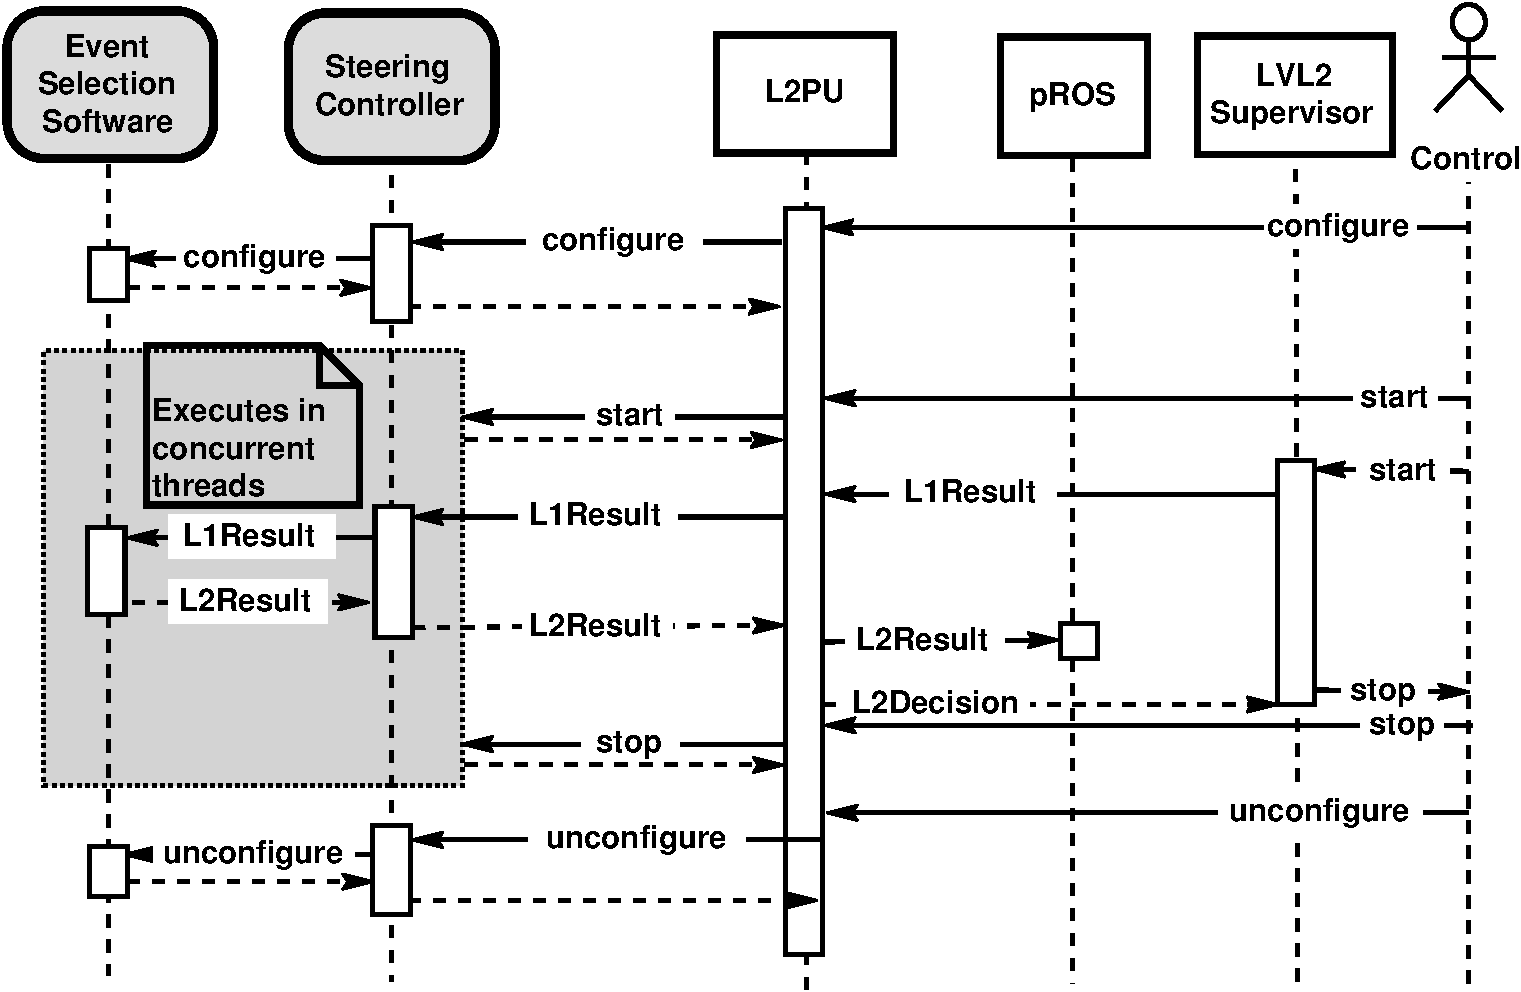
\includegraphics[scale=0.55]{tns2/2fig}
\end{center}
\caption{A seqüência de interações do L2SC com o L2PU e o \eng{software} de
seleção de eventos. Extraída de \cite{aa:tns-2004-2}.}
\label{fig:l2sc-interaction}
\end{figure}

Após a \textit{Inicialização} o L2SC recebe uma chamada \texttt{Execute Event}
com um resultado do LVL1 como argumento. O resultado do processamento do
evento é automaticamente retornado como resultado do LVL2 para a L2PU. O
comando \textit{Término} termina a execução dos algoritmos e produz um sumário
do período de execução.

\subsubsection{Modelo de desenvolvimento do L2SC}

Uma vez que as mesmas interfaces estão disponíveis no LVL2 e no EF, o código
desenvolvido no ambiente \eng{offline} pode ser diretamente carregado em seu
formato binário nestes processadores. Para o LVL2, no entanto, o desenvolvedor
deve seguir um conjunto de regras simples \cite{aa:lvl2-coding} durante o
ciclo de desenvolvimento para produzir código seguro ao acesso concorrente (do
inglês \eng{thread-safe}) ou serviços compatíveis com a criação automática de
múltiplas cópias na L2PU. Não deve ser necessário utilizar trancas
(\eng{locks}) ou \eng{mutexes} para adaptar o código a este ambiente
multi-tarefas. Para respeitar as restrições no tempo de execução para o LVL2, o
número e o tipo de serviços disponíveis estão restritos ao mínimo necessário,
sendo este um subconjunto do serviços disponíveis no EF e \eng{offline}. Desta
forma é sempre possível mover um componente do LVL2 para executar no EF ou até
\eng{offline}. A movimentação de algoritmos no sentido oposto, no entanto,
deve observar as restrições de operação no LVL2.

\subsubsection{Desempenho do HLT}

Após integrar, o L2SC com o Sistema de Fluxo de Dados, testes de desempenho e
robustez form conduzidos no CERN em uma máquina com dois núcleos tipo
AMD/Athon's de 1,533 GHz. O L2SC rodou por mais de 50 horas com três tarefas
processadoras. O protótipo executou sem problemas aparentes (\eng{dead-locks},
vazamentos de memória, etc.) em nós simples ou com dois núcleos,
mostrando a segurança ao acesso concorrente. Medidas do desempenho desta
infraestrutura exibiram um \eng{overhead} de 13 $\mu$s por evento. Este valor
foi estimado comparando-se o número de eventos por segundo que uma L2PU pode
manusear quando operando com e sem o L2SC e executando um algoritmo simples
(primeira e segunda linhas da Tabela~\ref{tab:l2sc}). Esta tabela também
mostra a taxa de processamento obtida quando, adicionalmente, o resultado do
LVL1 é transferido para o Gerente de Dados. O valor de \eng{overhead}
mencionado inclui toda a infraestrutura Athena para agendar e executar os
algoritmos e os serviços básicos. Estes valores são baseados em execuções de,
no mínimo, 100.000 eventos. Escalonamento quase perfeito da latência medida
foi observado quando o tempo de execução dos algoritmos era variado com um
ciclo de processamento fictício de 0 a 8 milissegundos em configurações
distintas, indicando que o \eng{overhead} por evento introduzido pelo L2SC é
independente do tempo de execução observado.

\begin{table}
\caption{Taxas de processamento em um sistema com dois núcleos tipo AMD-Athlon
1,533 GHz.} 
\label{tab:l2sc}
\begin{center}
\begin{tabular}{|l|c|c|}
\hline
Configuração do Protótipo & Taxa Medida & \eng{Overhead} por Evento \\
\hline
\hline
L2PU & 21,7 kHz & 46 $\mu$s \\
\hline
L2PU + L2SC & 17,0 kHz & 59 $\mu$s \\
\hline
L2PU + L2SC + Gerente de Dados & 15,3 kHz & 65 $\mu$s \\
\hline
\end{tabular}
\end{center}
\end{table}

Na seqüência, testes mais complexos foram feitos com uma fatia completa do
sistema de seleção para elétrons e fótons ($e^-/\gamma$). Estes testes
continham o Gerente do HLT, um algoritmo decodificador do resultado do LVL1,
agendamento de algoritmos para o LVL2 e o envio dos resultados do
processamento do LVL2 para o EF. O Gerente de Dados, o EDM e a descrição dos
detetores para os calorímetros do ATLAS foram também carregados no conjunto de
teste, que estava funcionando sobre uma bancada que consistia de três nós de
processamento: dois com dois núcleos (o AMD/Athlon anteriormente
mencionado e um Intel/Xeon de 2,2 GHz) hospedando o ROS e a L2PU
respectivamente, interconectados por
\eng{Gigabit} ethernet e um nó com apenas um processador (Intel/Pentium 4 de
2,2 GHz) para hospedar o L2SV. O algoritmo de extração de características para
dados do calorímetro foi especialmente desenvolvido para o LVL2, utilizando
toda a infraestrutura disponível mencionada anteriormente. Para este teste, 95
\% dos eventos foram processados em menos de 5 milissegundos para uma amostra
simulada de jatos duplos (\eng{di-jets}) em baixa luminosidade, para um
tamanho de RoI de $\Delta\eta \times \Delta\phi = 0,3 \times 0,3$. A
Figura~\ref{fig:l2sc-mu} exibe resultados similares para uma fatia completa de
seleção para múons. Nesta figura é possível, ver que as contribuições, em
ordem decrescente, para o tempo de processamento total de cada evento são
pré-processamento dos dados e sua conversão para o EDM, os \eng{overheads} da
infraestrutura provida pelo HLT (\eng{Steering}), processamento do algoritmo
de extração de características (denotado por \texttt{muFast} na figura) e o
tempo de acesso dos dados pela rede. As curvas mostram que, neste exemplo, o
processamento termina, para 95 \% dos eventos, em menos de 2 milissegundos. A
amostra de dados analisada consiste de múons com massa de 200 GeV em um
ambiente de alta luminosidade do feixe. Esta amostra, que é simulada através
de processos de Monte Carlo, inclui um ruído de fundo equivalente ao que será
observado na caverna do ATLAS em sua disposição final.

\begin{figure}
\begin{center}
\includegraphics[scale=0.65]{tns2/4fig}
\end{center}
\caption{As principais contribuições para o tempo de processamento mostradas
como integrais para a fatia completa do sistema de seleção para RoI's de
múons. Extraída de \cite{hlt-tdr}.}
\label{fig:l2sc-mu}
\end{figure}



\typeout{ *************** End of file trigger.tex *************** }
